\documentclass[11pt]{article}
\usepackage[english]{babel}
\usepackage[utf8]{inputenc}
\usepackage{fancyhdr}
\usepackage{graphicx}
\usepackage[colorlinks, linkcolor=blue, anchorcolor=blue, citecolor=blue]{hyperref}

\def\Name{Ran Liao}
\def\Topic{Life-Cycle Model}

\title{\textbf{\Topic}}
\author{\Name}
\markboth{Notes on \Topic\ }{Notes on \Topic\ }
\date{\today}
 
\pagestyle{fancy}
\fancyhf{}
\rhead{\date{\today} }
\lhead{Notes on \Topic\ }
\rfoot{\thepage}

\textheight=9in
%\textwidth=6.5in
\topmargin=-.75in
%\oddsidemargin=0in
%\evensidemargin=0in
 
\begin{document}
\maketitle
\noindent\makebox[\linewidth]{\rule[8pt]{5in}{0.5pt}}
 
\section*{Waterfall Model}

Waterfall model is characterized by its feedback loops and documentation-driven feature.
Due to the documentation, maintenance is easier.

\begin{figure}[h]
	\centering
	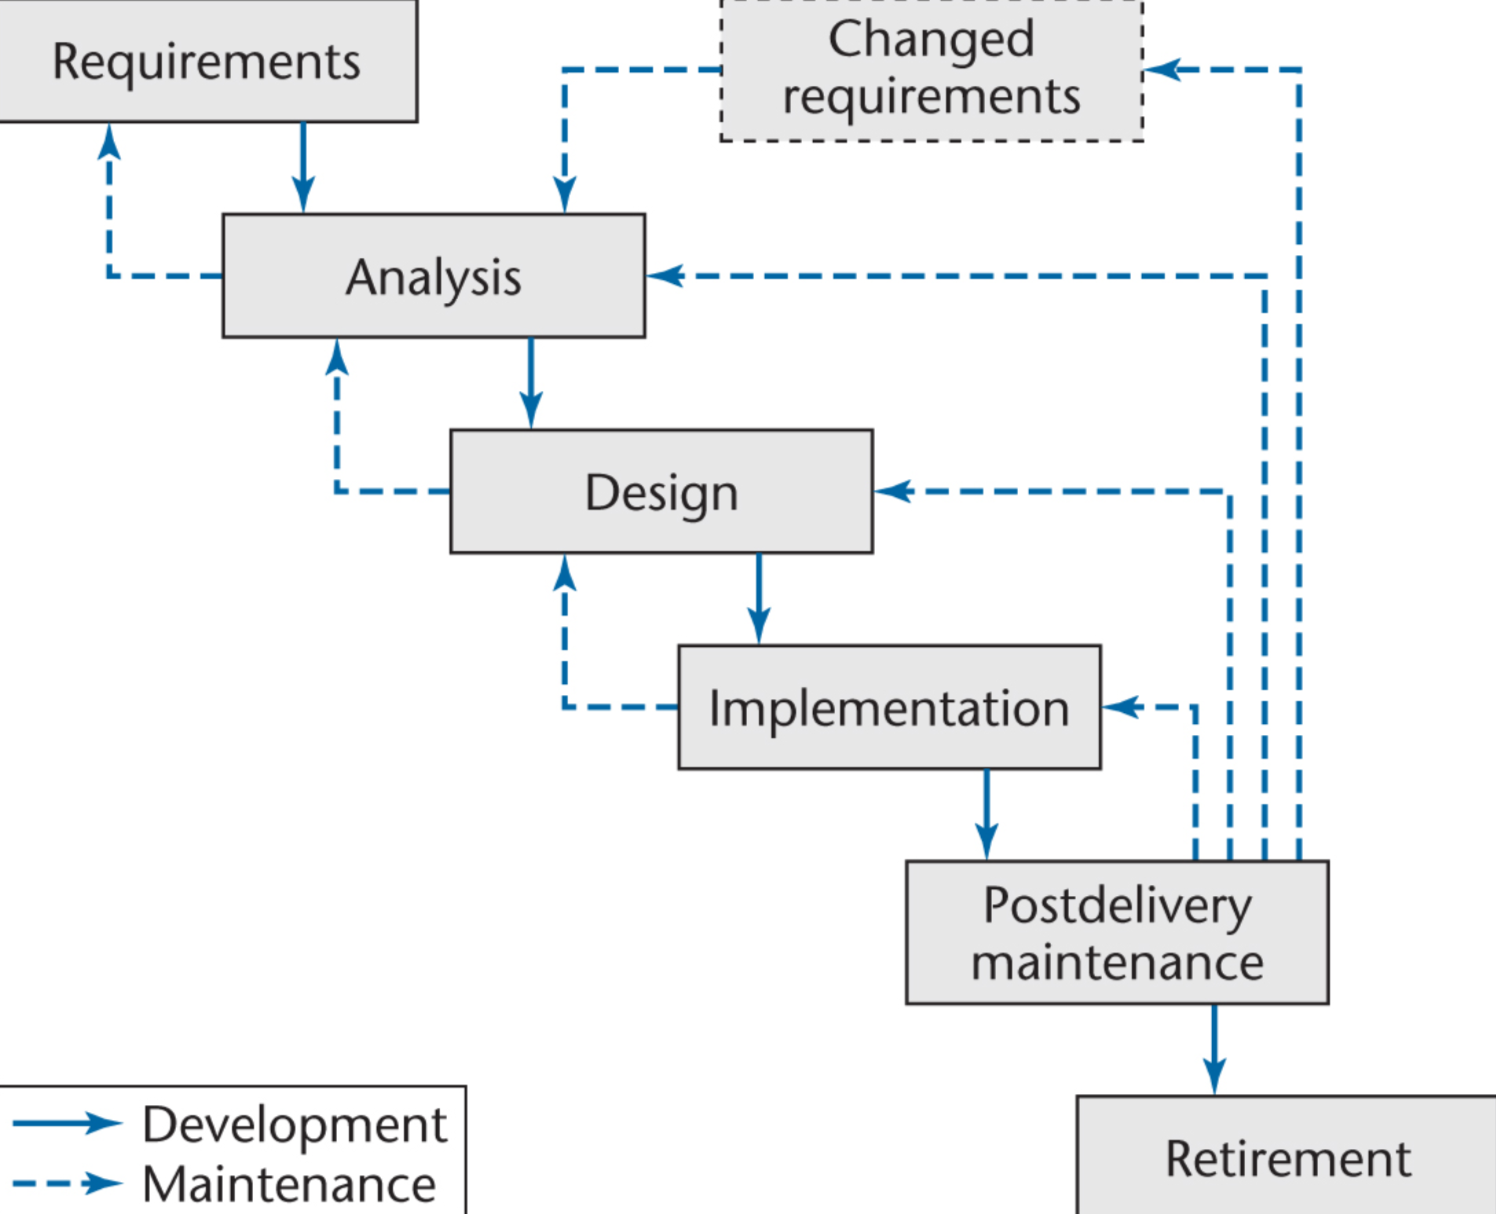
\includegraphics[width=0.6\linewidth]{images/Waterfall.png}
	\caption{Waterfall Model }
	\label{fig:Waterfall}
\end{figure}

\section*{Iteration and Incrementation Model}

The iterative-and-incremental life-cycle model is a model that applies waterfall model successively. Each increment is a waterfall mini project. Each successive version is intended to be closer to its target than its predecessor. The strengths of this model are as follows, 

\begin{enumerate}
	\item Since every iteration incorporates the test workflow, there are multiple opportunities for checking that the software product is correct. Therefore, faults can be detected and corrected early.
	
	\item The robustness of the architecture can be determined early in the life cycle.
	
	\item Risks can be mitigated (resolve) early.
	
	\item A working version of the software product is available from the start. And delivered partial versions can help smooth the introduction of the new product in the client organization
\end{enumerate}


\section*{Code-and-Fix Model}

There's no design process or specifications in this model. It is the easiest way to develop software, but also the the most expensive way in terms of maintenance.

\begin{figure}[h]
	\centering
	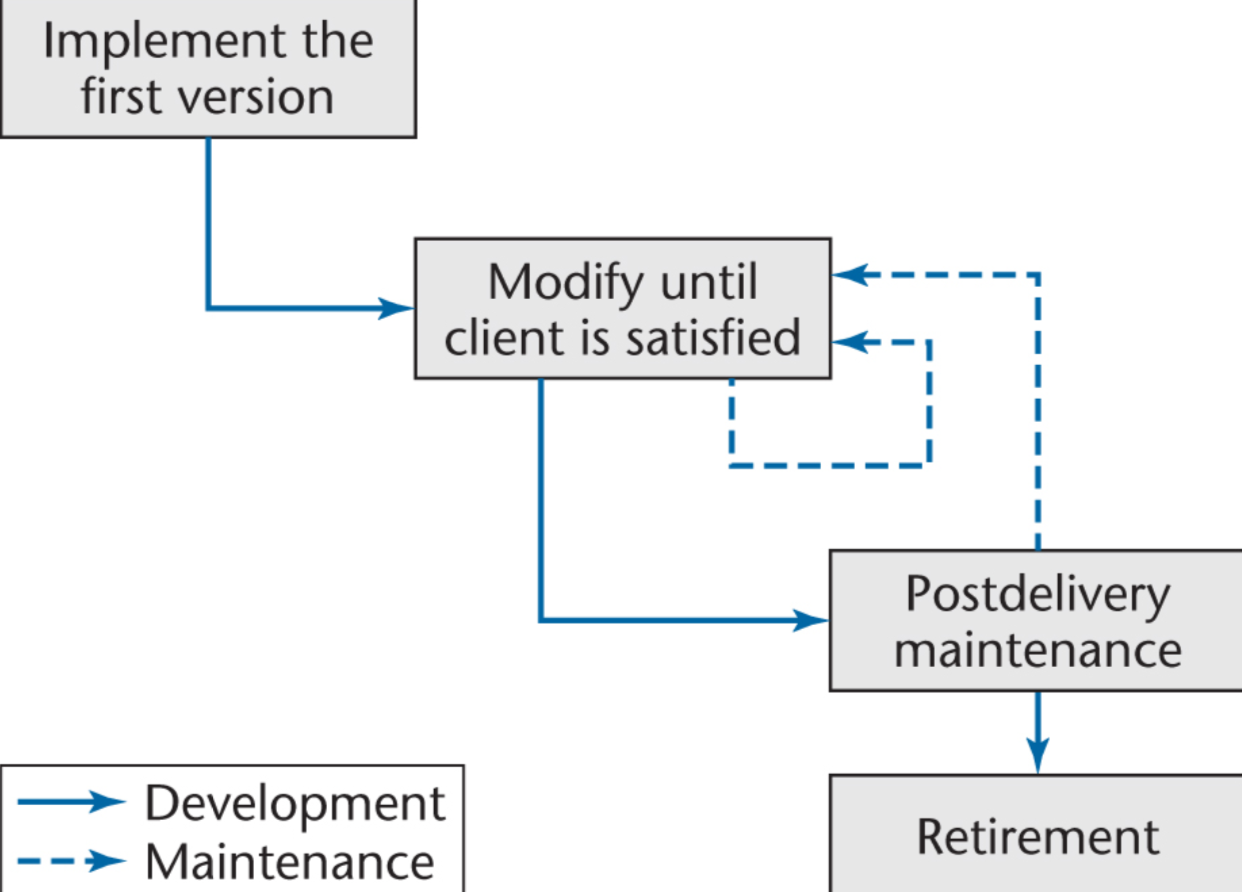
\includegraphics[width=0.6\linewidth]{images/CodeFix.png}
	\caption{Code-and-Fix Model }
	\label{fig:CodeFix}
\end{figure}

\section*{Rapid Prototyping Model}

\begin{figure}[h]
	\centering
	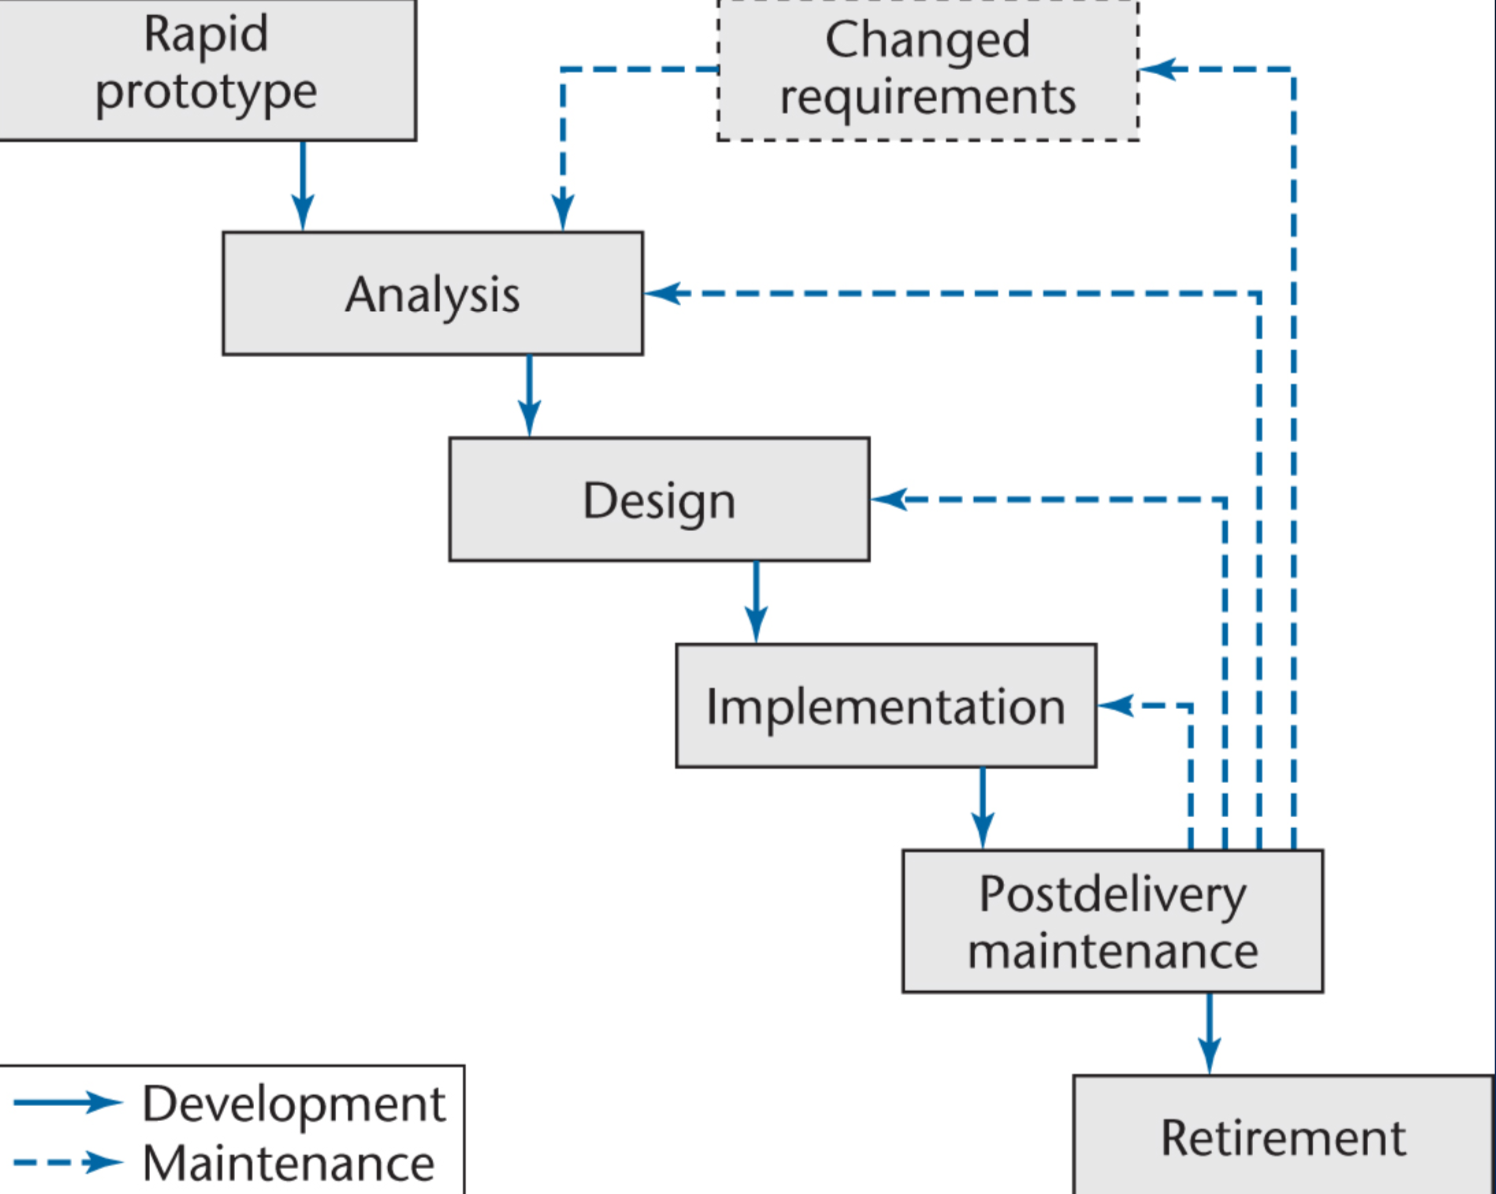
\includegraphics[width=0.6\linewidth]{images/RapidPrototyping.png}
	\caption{Rapid Prototyping Model }
	\label{fig:RapidPrototyping}
\end{figure}

\section*{Open-Source Life-Cycle Model}

There're two informal phases in this model. First, one individual builds an initial version and made available via the Internet. Then, if there is sufficient interest in the project, users become co-developers and the product is extended. In this model, individuals generally work voluntarily on the project in their spare time. 
The second informal phase consists solely of postdelivery maintenance including

\begin{itemize}
	\item Reporting and correcting defects (Corrective maintenance)
	\item Adding additional functionality (Perfective maintenance)
	\item Porting the program to a new environment (Adaptive maintenance)
\end{itemize}

\begin{figure}[h]
	\centering
	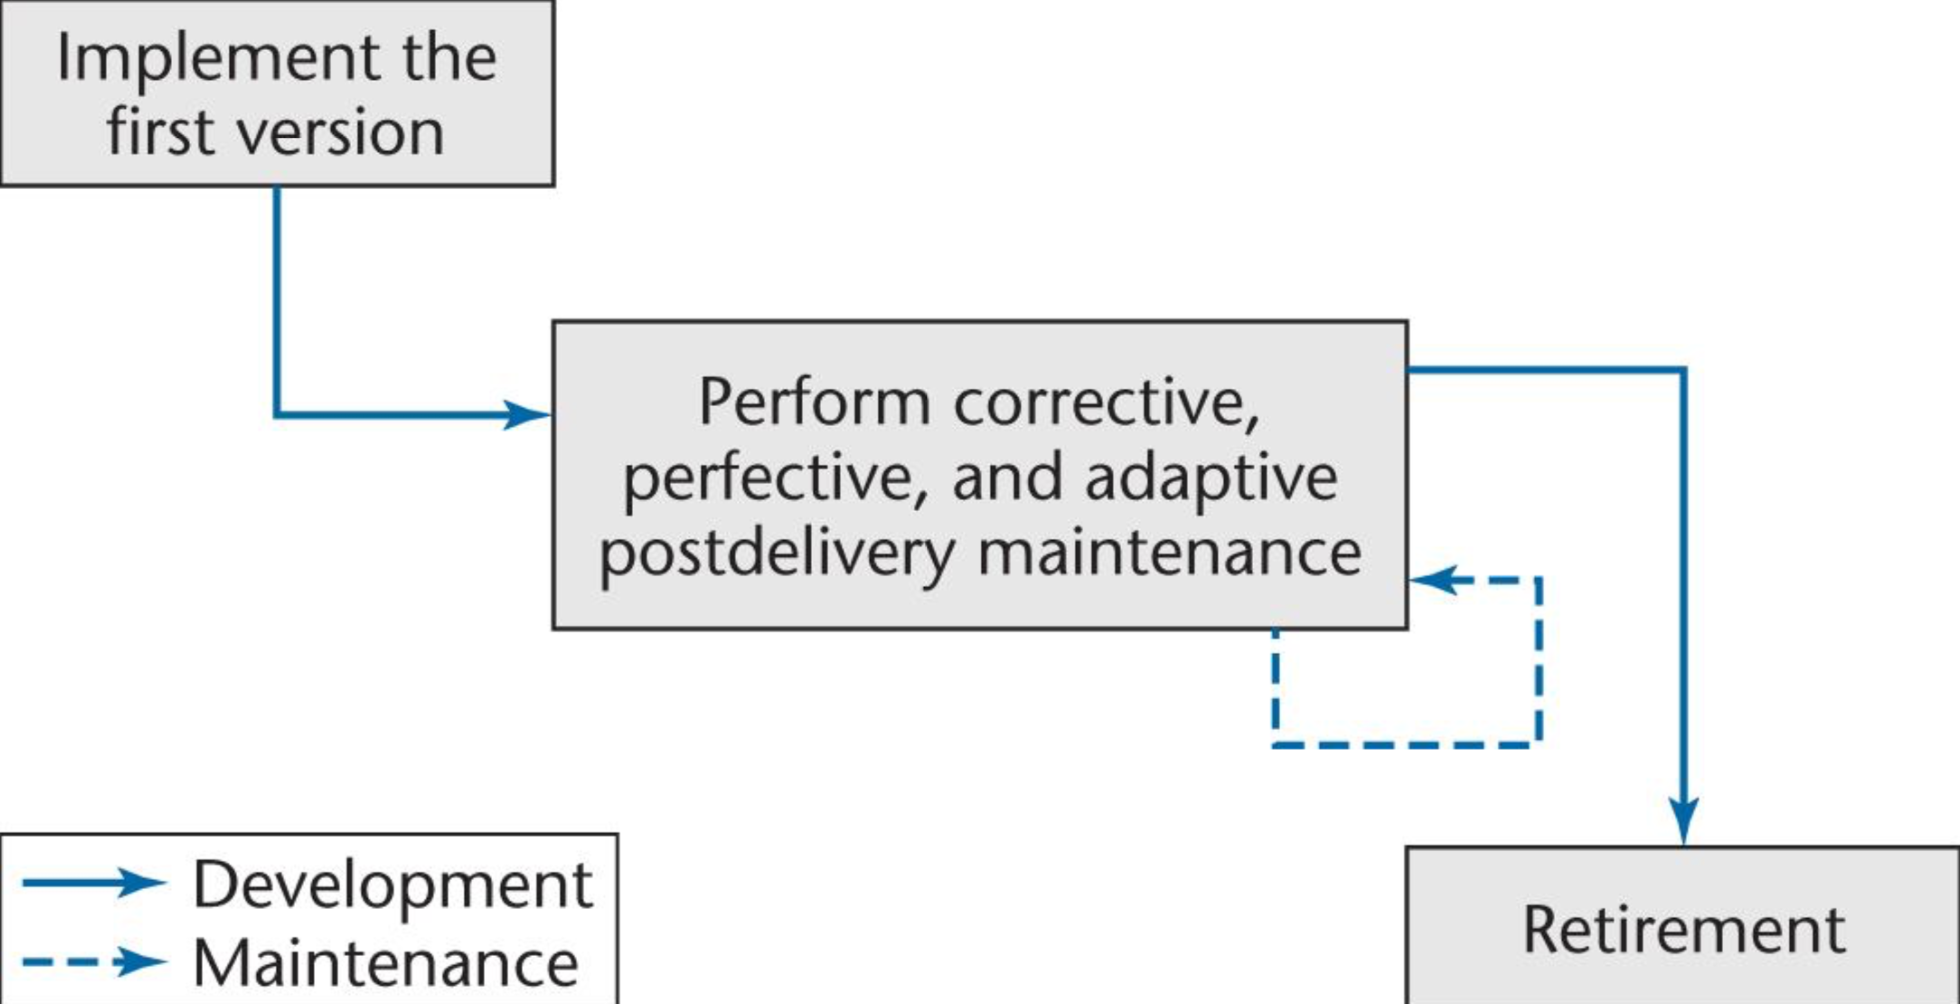
\includegraphics[width=0.6\linewidth]{images/OpenSource.png}
	\caption{Open-Source Model }
	\label{fig:OpenSource}
\end{figure}

The core group of an open-source software consists of a small number of dedicated maintainers with the inclination, the time, and the necessary skills to submit fault reports (“fixes”). They take responsibility for managing the project and have the authority to install fixes. Peripheral group consists of users who choose to submit defect reports from time to time.

Open-source softwares are a lot different from closed-source softwares. See Table ~\ref{tab:OpenSourceDiff} for details.
\begin{table}  
\caption{Difference between open-source software and closed-source software}  
\label{tab:OpenSourceDiff}
\begin{center}  
\begin{tabular}{p{5cm}|p{5cm}}  
\hline  
Open-source & Closed-source \\ \hline 
Maintained by unpaid volunteers. & Maintained and tested by employees.  \\ \hline  
Users are strongly encouraged to submit defect reports, both failure reports and fault reports. 
& Users can submit failure reports but never fault reports (the source code is not available).\\ \hline  
The core group releases a new version of an open-source product as soon as it is ready.
& New versions of closed-source software are typically released roughly once a year. \\ \hline  
Core group performs minimal testing. Extensive testing is performed by the members of the
peripheral group in the course of utilizing the software.
& Carefully tested by the SQA group. \\ \hline  
\end{tabular}  
\end{center} 
\end{table} 

An open-source project generally has no specifications and no design. Some open-source projects so successful because they have attracted some of the world’s finest software experts. Those experts can function effectively without specifications or designs.

When the open-source model has worked, it has sometimes been incredibly successful. However, the open-source life-cycle model is inapplicable unless the target product is viewed by a wide range of users as useful to them. In reality, about half of the open-source projects on the Web have not meet this requirement. Even where work has started, the overwhelming preponderance will never be completed.

\newpage
\section*{Agile Processes}

Agile processes are a collection of new paradigms characterized by
\begin{itemize}
	\item Less emphasis on analysis and design
	\item Earlier implementation (working software is considered more important than documentation)
	\item Responsiveness to change
	\item Close collaboration with the client
\end{itemize}

In agile processes, the team will deliver working software frequently, ideally every 2 or 3 weeks. Typically, 3 weeks for each iteration is set aside for a task. The team members then do the best job they can during that time.

Another common feature of agile processes is stand-up meetings. It's a short meeting that held at a regular time each day. During the meeting, participants stand in a circle. They do not sit around a table to ensure the meeting lasts no more than 15 minutes. The aim of a stand-up meeting is to raise problems, but not solve them. Solutions are found at follow-up meetings, preferably held directly after the stand-up meeting.

In conclusion, agile processes appear to be a useful approach to building small-scale software products when the client’s requirements are vague. Also, some of the proven features of agile processes can be effectively utilized within the context of other life-cycle models.

\section*{Synchronize-and Stabilize Model}

This is Microsoft’s life-cycle model. First, a requirements analysis is conducted. They may complete this through interview potential customers. Then they draw up specifications and divide project into 3 or 4 builds. Note that each build is carried out by small teams working in parallel. At the end of the day, they synchronize (test and debug) codes. At the end of the build, they stabilize (freeze) the build.

\section*{Spiral Model}

Spiral Model is simplified form rapid prototyping model plus risk analysis preceding each phase.

\begin{figure}[h]
	\centering
	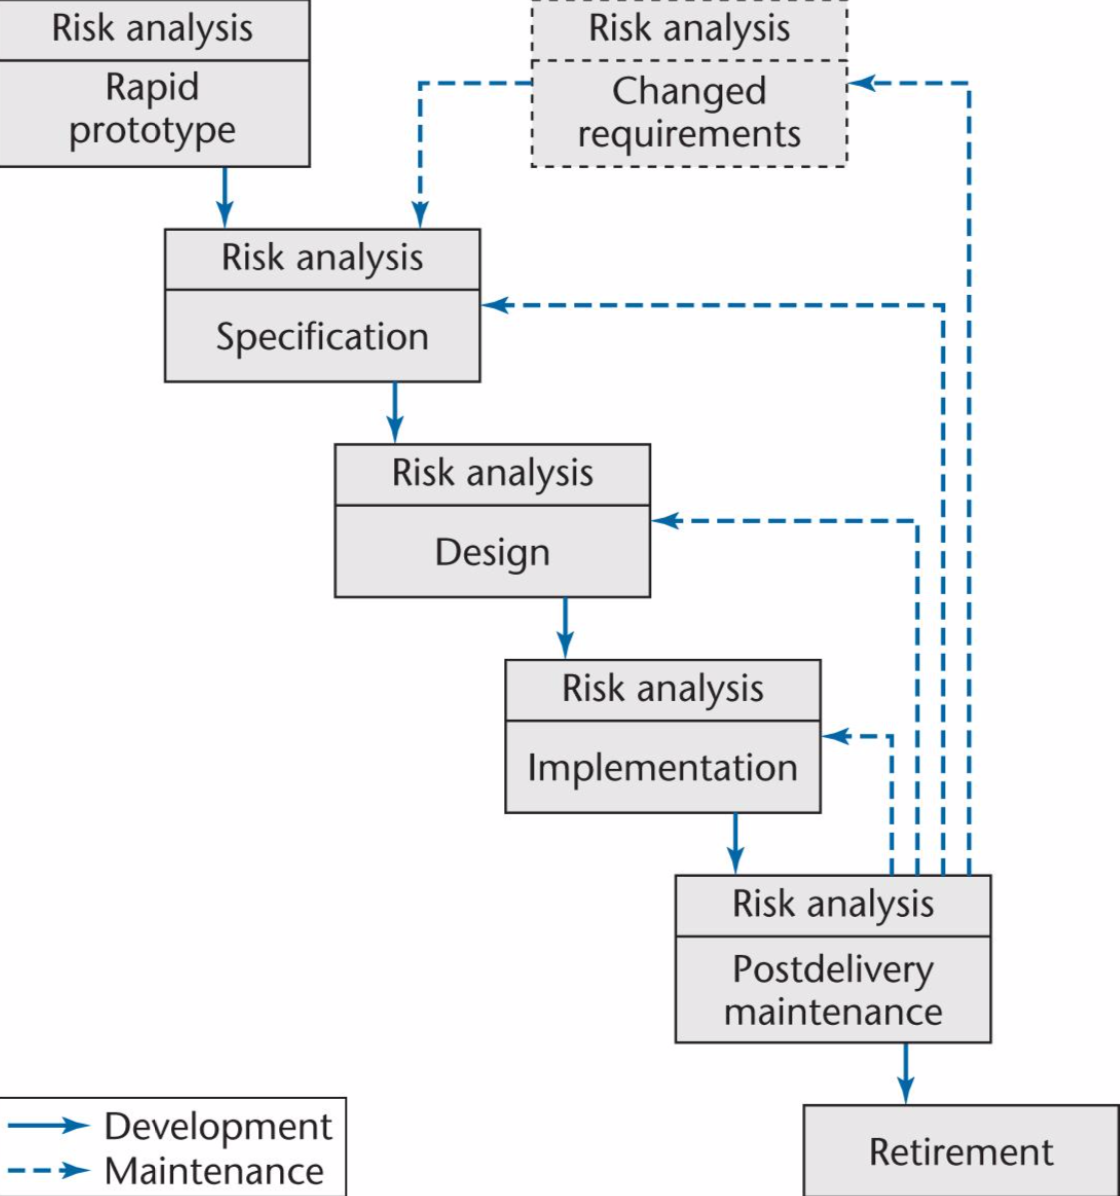
\includegraphics[width=0.4\linewidth]{images/Spiral.png}
	\caption{Spiral Model}
	\label{fig:Spiral}
\end{figure}

In full spiral model, each phase is preceded by alternatives and risk analysis. And each phase is followed by evaluation and planning of the next phase.

\begin{figure}[h]
	\centering
	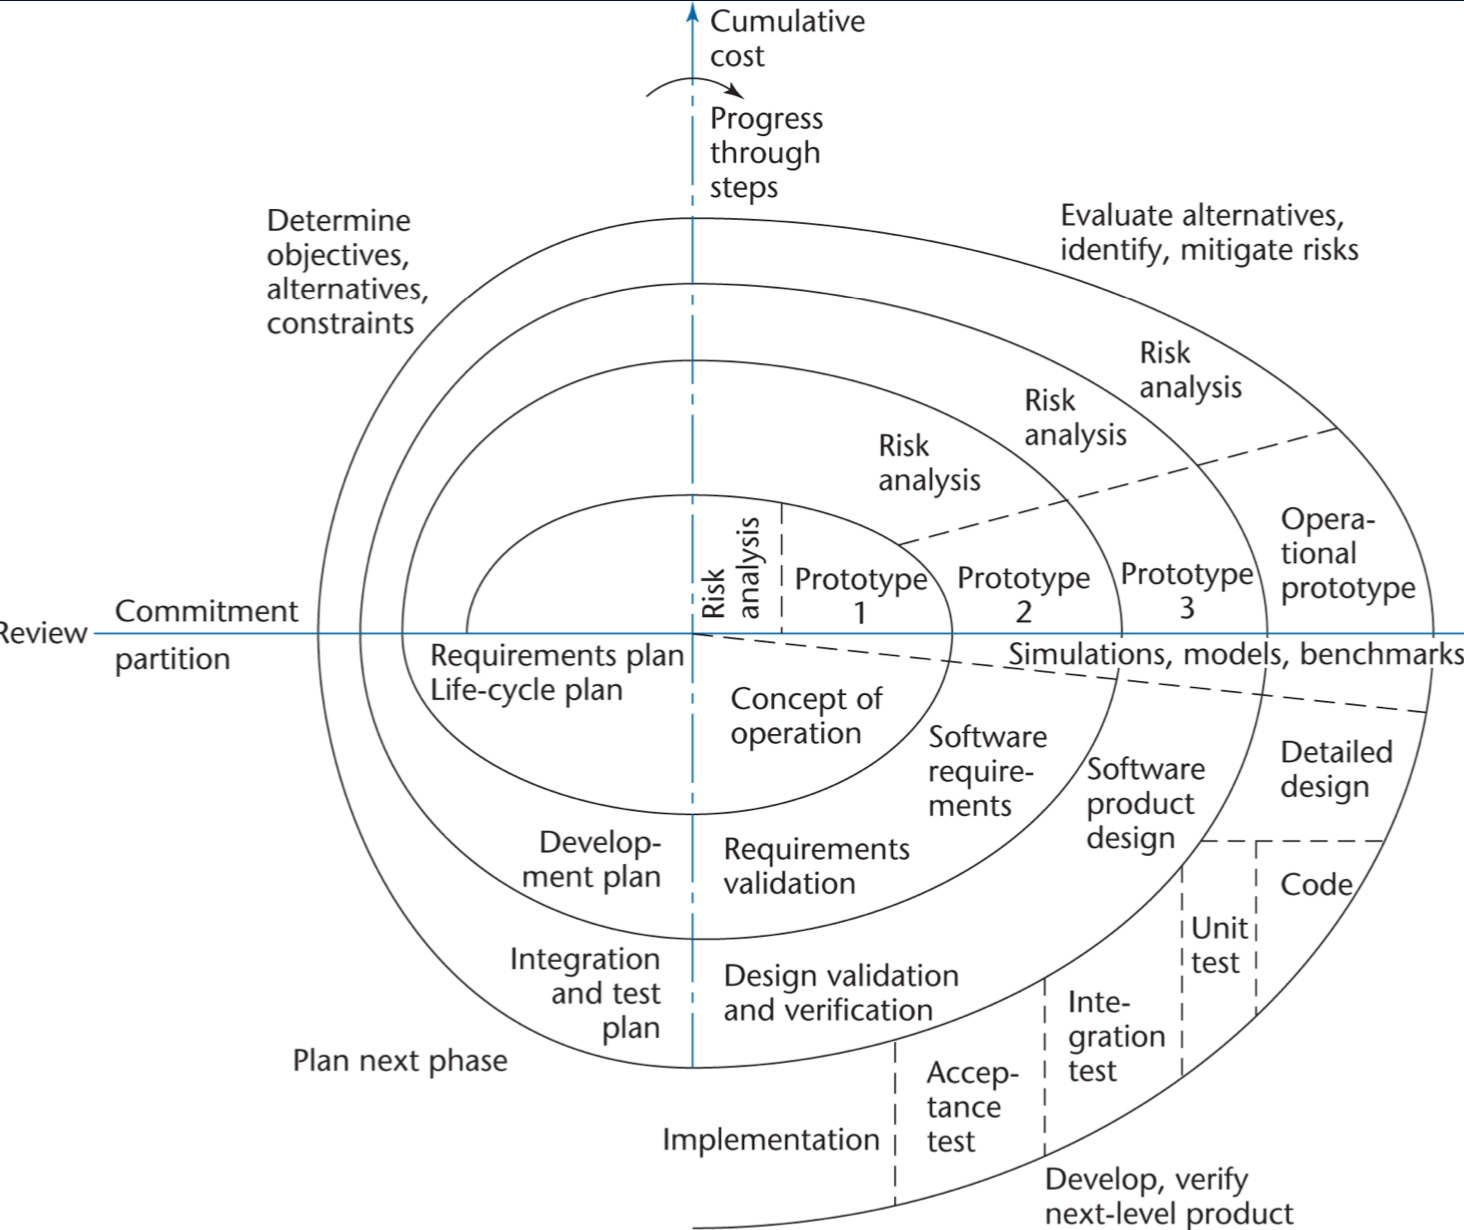
\includegraphics[width=0.6\linewidth]{images/FullSpiral.png}
	\caption{Full Spiral Model}
	\label{fig:FullSpiral}
\end{figure}

\section*{Evolution-Tree Model}
\begin{figure}[h]
	\centering
	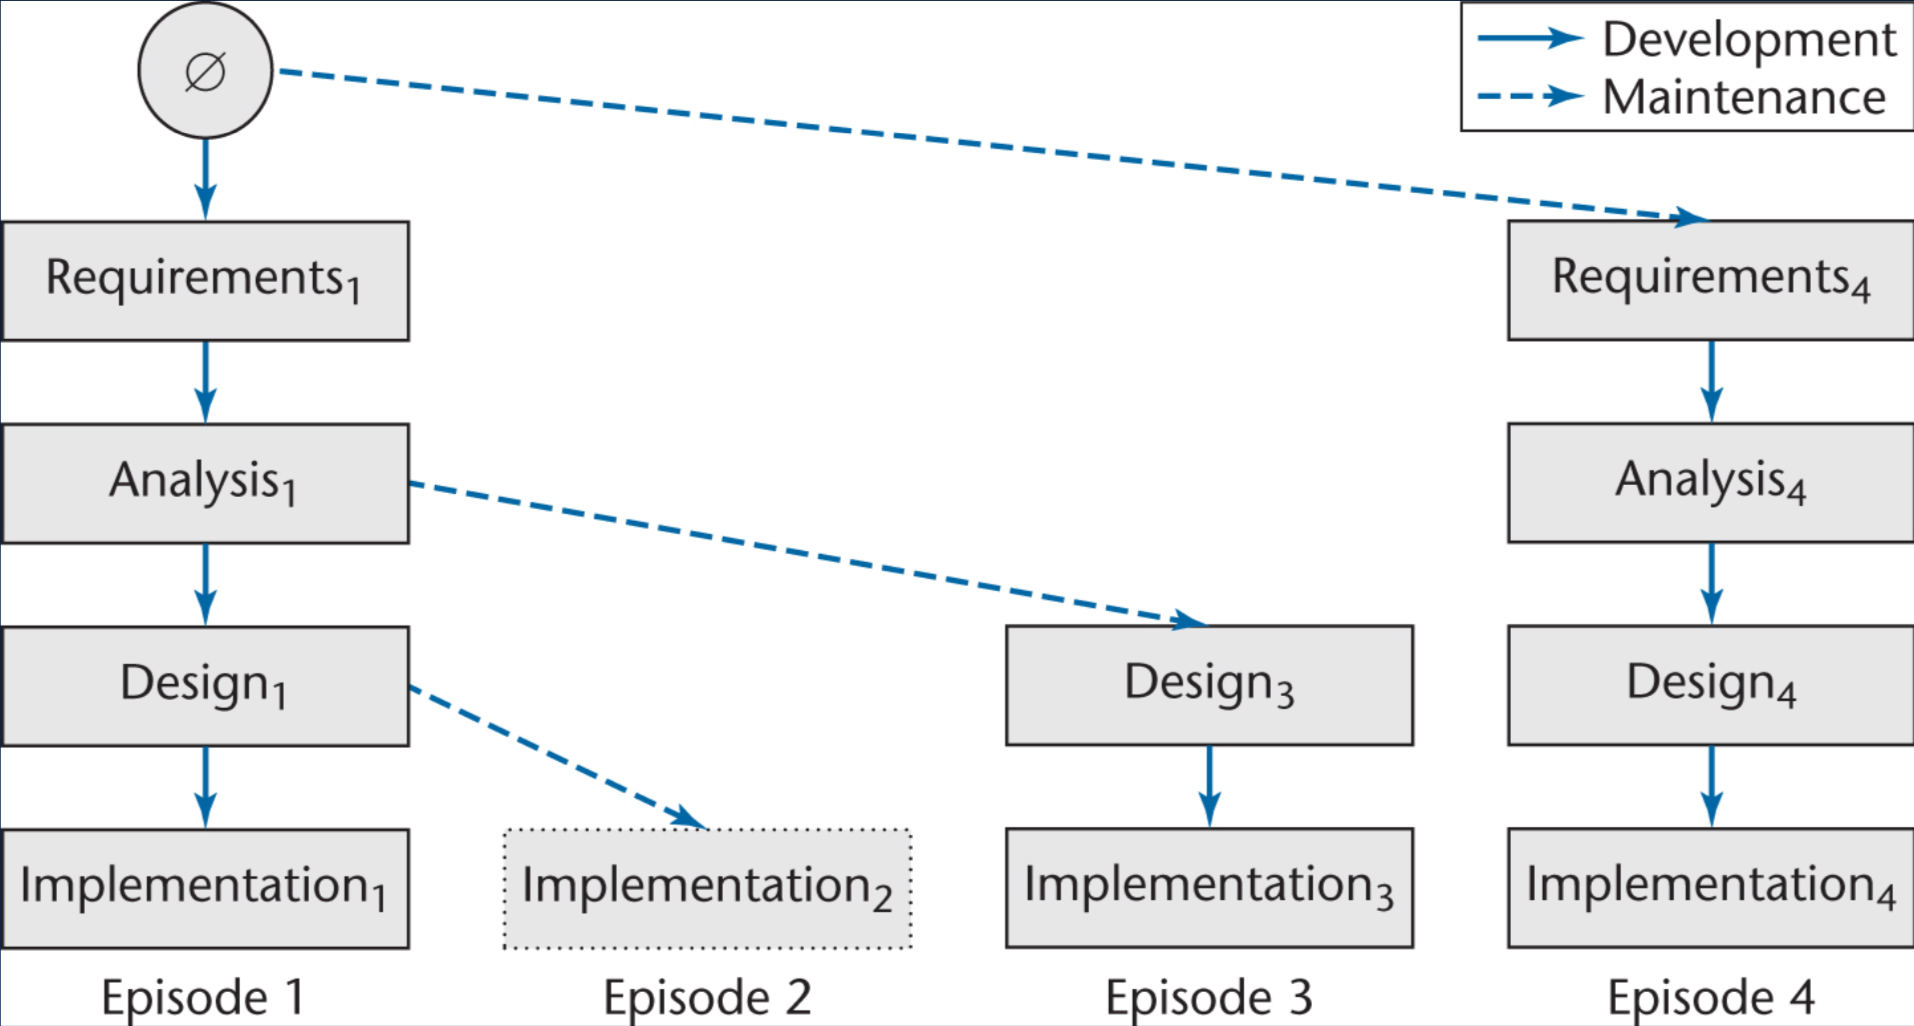
\includegraphics[width=0.8\linewidth]{images/EvolutionTree.png}
	\caption{Evolution-Tree Model}
	\label{fig:EvolutionTree}
\end{figure}

\section*{Comparison of Life-Cycle Models}
\begin{figure}[h]
	\centering
	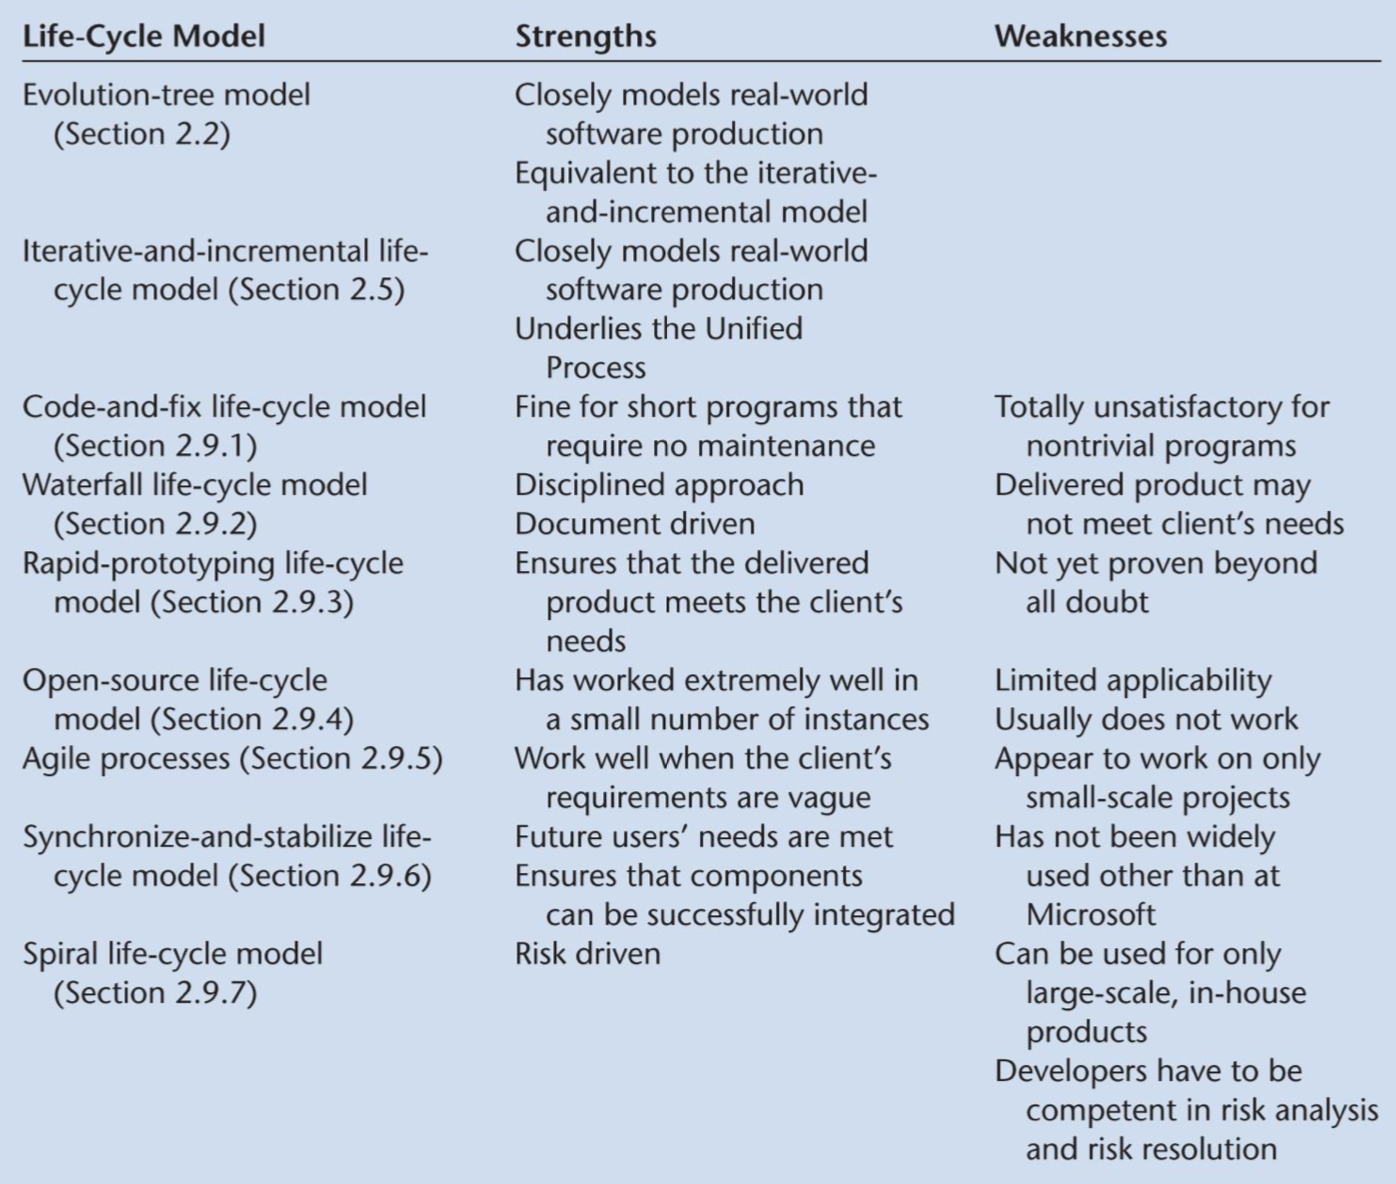
\includegraphics[width=0.9\linewidth]{images/Comparison.png}
	\caption{Comparison of Life-Cycle Models}
	\label{fig:Comparison}
\end{figure}

\end{document}